%!TEX root = main.tex
\section{Methods\label{sec:methods}} 
\subsection{Motivation}
\par We adopted a mixed methods research methodology that draws inspiration from ethnographic methods, iterative and participatory design, and controlled studies~\cite{miller_salkind_miller_2002,shneiderman2006strategies,Muller1993} to understand how VQSs can be used for scientific data analysis. Working with researchers from three different scientific research groups, we identified the needs and challenges of scientific data analysis and the potential opportunities for VQSs, via interviews and cognitive walkthroughs. 
\par Visualization systems are often evaluated using controlled studies that measure the user's performance against an existing visualization baseline~\cite{Plaisant2004}. Techniques such as artificially inserting ``insights'' or setting predefined tasks for example datasets work well for objective tasks, such as debugging data errors~\cite{kandel2011wrangler,Patel2010}, but these contrived methods are unsuitable for trying to learn about the types of real-world queries users may want to pose on VQSs. Due to the unrealistic nature of controlled studies, many have proposed using a more multi-faceted, ethnographic approach to understand how analysts perform visual data analysis and reasoning~\cite{Plaisant2004,lam2012empirical,shneiderman2006strategies,munzner2009nested,Sedlmair2012}. In order to make the user study more realistic, we opted for a qualitative evaluation where we allowed participants to bring datasets that they have vested interests in to address unanswered research questions. Participatory design has been successfully used in the development of interactive visualization systems in the past~\cite{Aragon2008,Chuang2012}. Sedlmair et al. \cite{Sedlmair2012} advocate that design study methodology is suitable for use cases in which the data is available for prototyping, but the task is only partially known and the information is partially in the user's head. In that regard, our scientific use cases with VQS is well-suited for a design study methodology, as we learn about the scientist's data and analysis requirements and design interactions that helps users translate their ``in-the-head'' specifications into actionable visual queries.
\subsection{Participatory Design}
\par We recruited participants by reaching out to research groups via email and word of mouth, who have experienced challenges in dealing with large amounts of data. We initially spoke to analysts from 12 different potential application areas and narrowed down to three use cases in astronomy, genetics, and material science for our participatory design study. Six scientists from three research groups participated in the design of \zv. On average, the participants had more than 8 years of research experience working in their respective fields. We list the participants in Table~\ref{participants}, and will refer to them by their anonymized ID as listed in the table throughout the paper. 
\par Our initial inspiration for building a VQS came from informal discussions with academic and industry analysts. Their current workflows required analysts to manually examine large numbers of visualizations to derive insights from their data. Given these early conversations with the participants, we built a basic VQS to serve as the functional prototype in the design study. As shown in Figure \ref{oldZV}, this early version of \zv allowed users to sketch a pattern or drag-and-drop an existing visualization as a query,then the system would return visualizations that had the closest Euclidean distance from the queried pattern. The details of the system is described in our previous work \cite{Siddiqui2017,Siddiqui2017VLDB}, which focused on the systems and scalability aspects of the VQSs.
	\begin{figure}[ht!] 
	\centering
	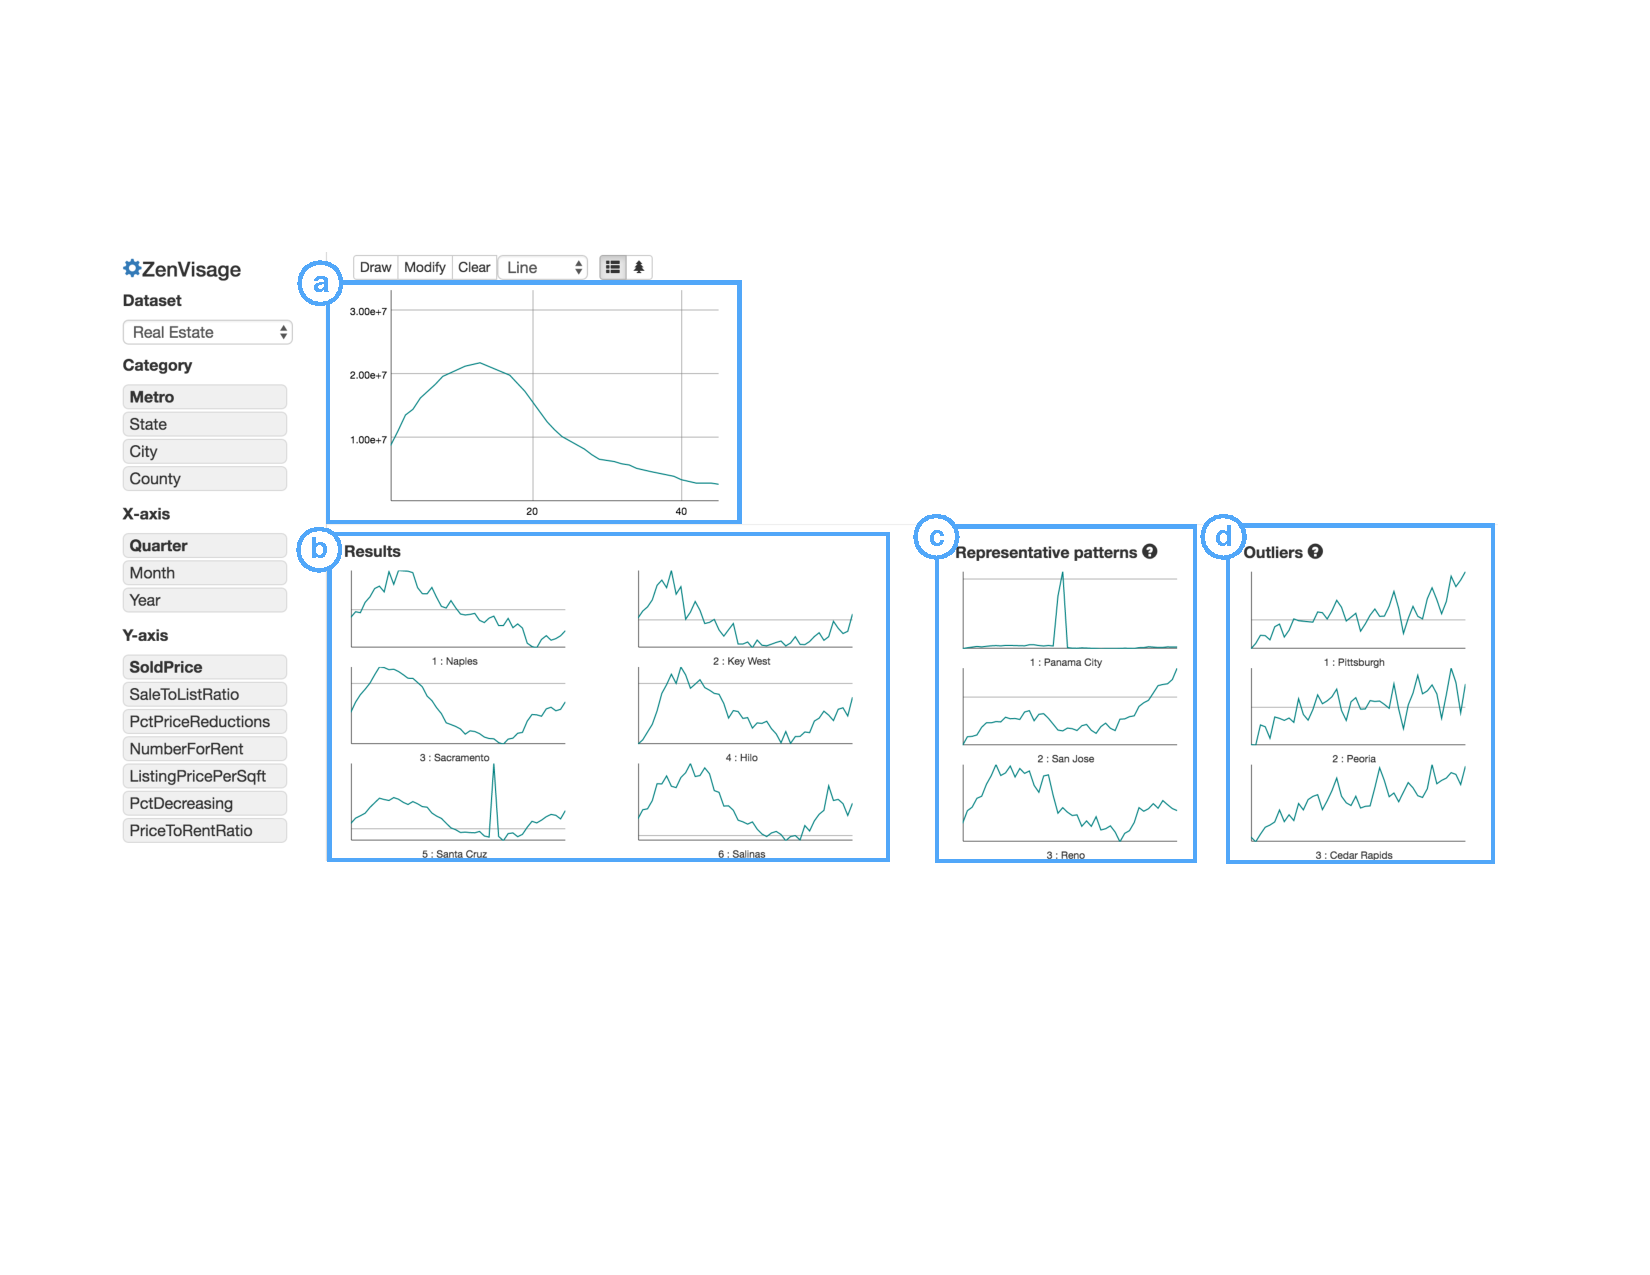
\includegraphics[width=\linewidth]{figures/oldZV_nozql.pdf}
	\caption{The \zv prototype allowed users to sketch a pattern in (a), which would then return (b) results that had the closest Euclidean distance from the sketched pattern. The system also displays (c) representative patterns obtained through K-Means clustering and (d) outlier patterns to help the users gain an overview of the dataset.}
	\label{oldZV}
	\end{figure}
\par The use of functional prototypes is common in participatory design to provide a starting point for the participants. For example, Ciolfi et al.\cite{Ciolfi2016} studied two different alternatives to co-design (starting with open brief versus functional prototype) in the development of museum guidance systems and found that while both approaches were equally fruitful, functional prototypes can make addressing a specific challenge more immediate and focused. Our motivation for providing a functional prototype at the beginning of the participatory design sessions is to showcase capabilities of VQSs. Especially since VQSs are not common in the existing workflows of these scientists, participants may not be able to imagine their use cases without a starting point. 
\par During the participatory design process, we collaborated with each of the teams closely with an average of two meetings per month, where we learned about their datasets, objectives, and how VQSs could help address their research questions. A detailed timeline of our engagement with the participants and the features inspired by their use cases can be found in Figure \ref{timeline}. Participants provided datasets they were exploring from their domain, whereby they had a vested interest in using a VQS to address their own research questions. Through this process, we identified and incorporated more than 20 desired features into the VQS prototype over the period of a year. 
\begin{figure*}[!ht]
	\centering
	\captionsetup{justification=centering,margin=2cm}
	\vspace{-10pt}
	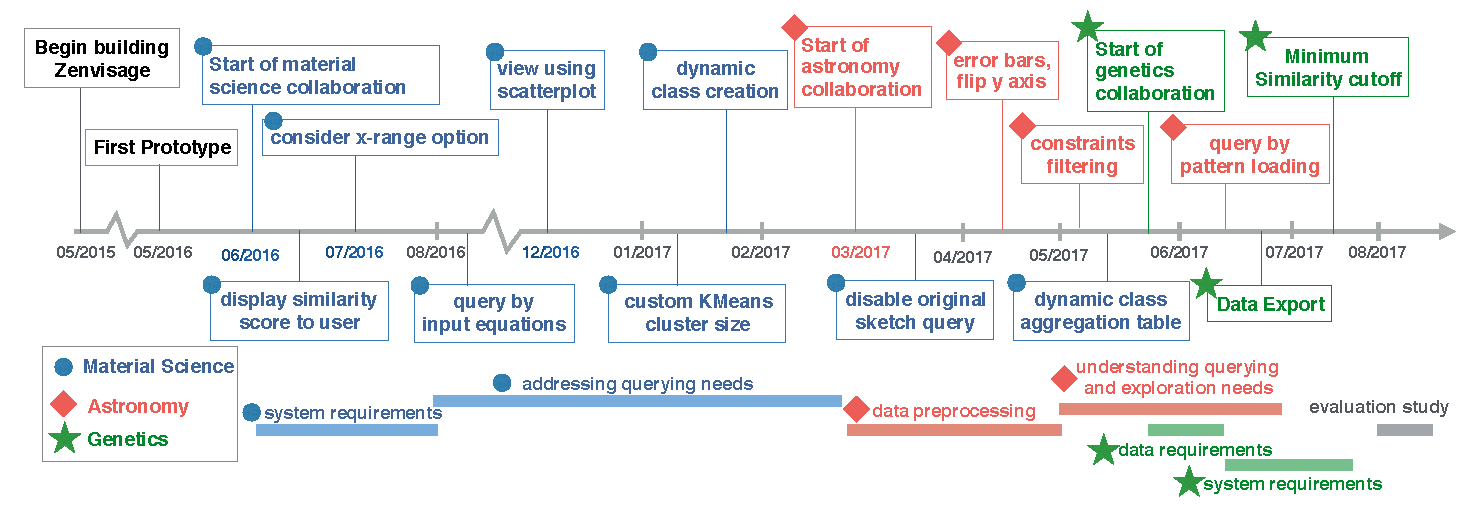
\includegraphics[width=6in]{figures/timeline_new.pdf}
	\vspace{-6pt}\caption{Participatory design timeline for the scientific use cases.}
	\label{timeline}
	\vspace{-10pt}
\end{figure*}
\subsection{Evaluation Study}
\par Finally, we conducted a realistic, qualitative evaluation to study how analysts interact with different VQS components in practice. The evaluation study participants included the six scientists from the participatory design study, along with three additional ``blank-slate'' participants who had never encountered \zv before. While participatory design subjects actively provided feedback on \zv with their data, they only saw us demonstrating their requested features and explaining the system to them, rather than actively using the system on their own. So the evaluation study was the first time that all nine of the participants used \zv to explore their datasets.
\par Participants for the evaluation study were recruited from each of the three aforementioned research groups, as well as domain-specific mailing lists. Prior to the study, we asked the potential participants to fill out a pre-study survey to determine their eligibility. Eligibility criteria included: being an active researcher in the subject area with more than one year of research experience, and having worked on a research project involving data of the same nature as that used in the participatory design. Four of the user studies were conducted remotely.  
\par Participants had the option of exploring their own dataset or an existing dataset that they provided to us during the participatory design process. All three blank-slate participants opted to explore their own datasets. After loading their dataset, we emailed them a screenshot of a visualization from our tool to verify that we configured the system to meet their needs. 
\par At the start, participants were provided with an interactive walk-through explaining the details of the features offered in our VQS. The participants were then given approximately ten minutes to experience a guided exploration of our VQS with a preloaded real-estate example dataset from Zillow \cite{zillow}.\techreport{This dataset contained housing data for various cities, metropolitan areas, and states in the U.S. from 2004-15.} After familiarizing themselves with the tool, we loaded the participant's dataset and suggested an appropriate choice of axis to begin the exploration. Participants were encouraged to talk-aloud during the data exploration phase.
\par During the exploration phase, participants were informed that they could use other tools as needed. If the participant was out of ideas\ccut{ for three minutes}, we suggested one of the ten main functionalities in \zv \techreport{\footnote{query by sketching, drag-and-drop, pattern loading, input equations, representative and outliers, narrow/ignore x-range options, filtering, data smoothing, creating dynamic classes,  data export}}that they had not yet covered. If any of these operations were not applicable to their specific dataset, they were allowed to skip the operation after having considered how it may or may not be applicable to their workflow. The user study ended after they covered all ten main functionalities. On average, the main exploration phase lasted for 63 minutes. After the study, we asked them open-ended questions about their experience. 
